\documentclass[../Head/Main.tex]{subfiles}
\begin{document}
\begin{figure}[H]
	\begin{subfigure}[b]{0.49\textwidth}
		\centering
		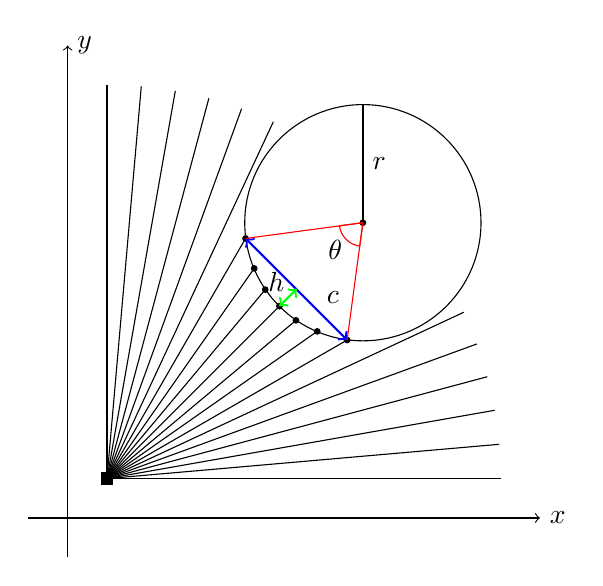
\begin{tikzpicture}
			\draw [->](0,-0.5)--(0,6) node[right]{$y$};
			\draw [->](-0.5,0)--(6,0) node[right]{$x$};
			\filldraw (0.425,0.425) rectangle (0.575,0.575);
			\draw (3.75,3.75) circle(1.5);
			\filldraw (2.69, 2.69) circle (1pt);
			\filldraw (2.51, 2.9) circle (1pt);
			\filldraw (2.37, 3.17) circle (1pt);
			\filldraw (2.26, 3.55) circle (1pt);
			\filldraw (3.55, 2.26) circle (1pt);
			\filldraw (3.17, 2.37) circle (1pt);
			\filldraw (2.9, 2.51) circle (1pt);		
			\filldraw (3.75, 3.75) circle (1pt);		
		
			\draw (0.5,0.5) -- (2.69, 2.69);
			\draw (0.5,0.5) -- (2.51, 2.9);
			\draw (0.5,0.5) -- (2.37, 3.17);
			\draw (0.5,0.5) -- (2.26, 3.55);
			\draw (0.5,0.5) -- (3.55, 2.26);
			\draw (0.5,0.5) -- (3.17, 2.37);
			\draw (0.5,0.5) -- (2.9, 2.51);
			\draw[blue, thick, <->] (2.26, 3.55) -- (3.55, 2.26);
			\draw[green, thick, <->] (2.69,2.69) -- (2.91, 2.91);
			\draw[thick] (3.75,3.75) -- (3.75, 5.25);
			
			\draw (0.5,0.5) -- (2.613, 5.032);	
			\draw (0.5,0.5) -- (2.21, 5.198);
			\draw (0.5,0.5) -- (1.794, 5.33);
			\draw (0.5,0.5) -- (1.368, 5.424);
			\draw (0.5,0.5) -- (0.9358, 5.481);
			\draw (0.5,0.5) -- (0.5, 5.5);
			
			\draw (0.5,0.5) -- (5.032, 2.613);	
			\draw (0.5,0.5) -- (5.198, 2.21);
			\draw (0.5,0.5) -- (5.33, 1.794);
			\draw (0.5,0.5) -- (5.424, 1.368);
			\draw (0.5,0.5) -- (5.481, 0.9358);
			\draw (0.5,0.5) -- (5.5, 0.5);
		
			\draw[red] (2.26, 3.55) -- (3.75, 3.75);
			\draw[red] (3.55, 2.26) -- (3.75, 3.75);
			\draw[red] (3.75, 3.75) -- +(-97.53:0.3) arc(-97.53:-172.47:0.3) -- cycle;
		
			\node[right] at (3.75,4.5) {$r$};
			\node at (2.65,3) {$h$};
			\node[right] at (3.17, 2.8) {$c$};
			\node at (3.4,3.4) {$\theta$};
		\end{tikzpicture}
		\caption{Illustration of detected points (marked as ending point of the black lines), the circle chord and arch heigh can be found from the LIDAR data}
		\label{fig:lidar_marble_detec}
  	\end{subfigure}
  	\hfill
  	\begin{subfigure}[b]{0.49\textwidth}
		\centering
		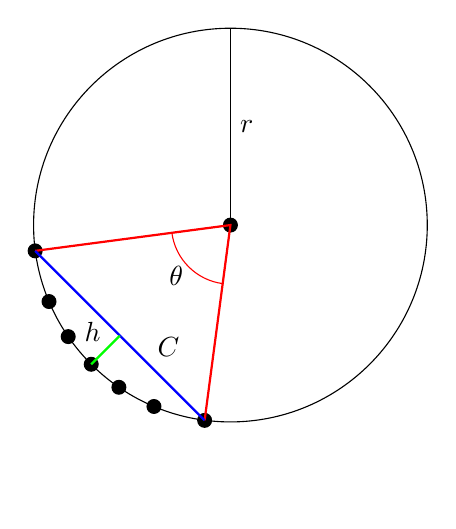
\begin{tikzpicture}
			\draw (3.5, 3.5) -- (3.5, 6);
			\draw (3.5, 4.75) node[right]{$r$};
			\draw [red] (3.5, 3.5) -- +(-97.53:0.75) arc(-97.53:-172.47:0.75) -- cycle;
			\draw (2.6, 2.85) node[right]{$\theta$};
			\draw (2.45, 1.95) node[right]{$C$};
			\draw (1.75, 1.9) node[above]{$h$};
			\draw (3.5, 3.5) circle (2.5);
			\filldraw (3.5,3.5) circle (2.5pt);
			\filldraw (1.7322,1.7322) circle (2.5pt);
			\filldraw (1.02, 3.1724) circle (2.5pt);
			\filldraw (3.1724, 1.02) circle (2.5pt);
			\filldraw (1.1962,2.529) circle (2.5pt);
			\filldraw (2.529,1.1962) circle (2.5pt);
			\filldraw (1.4399,2.0836) circle (2.5pt);
			\filldraw (2.0836,1.4399) circle (2.5pt);
			\draw [red, thick] (3.1724, 1.02) -- (3.5, 3.5) -- (1.02, 3.1724);
			\draw [blue, thick] (3.1724, 1.02) -- (1.02, 3.1724);
			\draw [green, thick] (1.7322, 1.7322) -- (2.096, 2.096);
			\draw [white] (3.5, 0);
		\end{tikzpicture}
		\caption{Illustration of the circle chord and arch heigh can be found from the LIDAR data and thereby can determine the circle's radius and the chord angle}
		\label{fig:lidar_marble_scaled}
  	\end{subfigure}
  	\vspace{-5pt}
  	\caption{Illustration of determination of the circle radius from LIDAR data}
  	\label{fig:lidar_marble}
  	\vspace{-15pt}
\end{figure}
\end{document}